\chapter{Design and Implementation}

\section{Development Methodology}
Software development methodologies break the development of a piece of software down into a number of phases with the aim of improving design and code quality as well as aiding in project management. There are a large number of different development methodologies, although they can typically be classified as either sequential, also called waterfall, or cyclical, also called spiral. The choice of which method to use will depend on the specifics of the software project as well as developer preference and team size.

\subsection{Sequential}
The sequential, or waterfall, approach uses a number of strict, sequential phases for developing software; each phase must be completed before the next phase can begin. Fig. \ref{fig:waterfall} shows the typical structure of this methodology.
\begin{figure}[tp]
   \begin{center}
     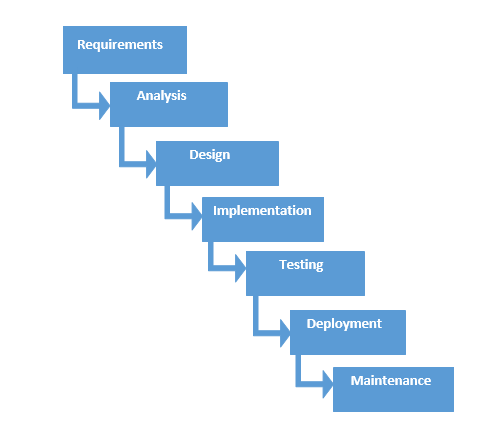
\includegraphics{Figures/waterfall.png}
   \end{center}
   \caption[Waterfall development methodology]{Waterfall development methodology \parencite{Naveen}}
   \label{fig:waterfall}
\end{figure}
\\This approach works well for projects were the requirements are strictly defined, the project's subject area well known and the technologies involved well understood by the developers. In this case, the software can be designed well from the start, so there is little need for iterative development. If the project's requirements are likely to change, or the subject area and technologies are ill-understood or new then a waterfall approach is inappropriate. The rigid structure of the waterfall method does not allow requirements to be easily changed, or poor design choices corrected; in order to change requirements or correct poor design the whole development process must be started again, as there is no method of feedback between development phases.

\subsection{Cyclical}
Cyclical approaches, as the name suggests, develop software using iterative cycles. At the start of each cycle requirements and design are set and at the end, a working software prototype is produced. This prototype is used as feedback for the next cycle, adjusting the requirements and correcting design mistakes and issues as necessary. These methods counteract the disadvantages of the waterfall approach; by using an iterative approach it is easy to add or change requirements or redesign areas of the project.
\\There are many development methods which are derived from a cyclic approach, including Rapid Application Development (RAD) and Scrum.
\\RAD is a development method which favours rapid prototyping with minimal planning. Since there is less focus on planning at each iteration it is extremely easy to incorporate design and requirement changes. Prototype development will start earlier than other methods and this enables issues to be caught early, and the design to be altered appropriately. There is a requirement when using RAD of skilled and experience developers and designers, as the prototypes  developed must be reusable so as to avoid wasting time.
\\Using Scrum, a project is broken down into sprints and each sprint is timeboxed with a duration, i.e. 24 hours, 4 weeks. At the end of each sprint a working prototype is produced and as the sprints are completed the project is designed and developed over time.

\subsection{Chosen Methodology}
For this project, cyclical methods were preferred over waterfall. This was partly due to the author's preference for cyclical methods and partly because there were some unknowns, particularly related to rendering, that made rigidly designing the system difficult. Using the more agile cyclical methods allowed for some investigative work before finalising the system design.
\\In particular, RAD was chosen as the development methodology.

\section{Development}
Since RAD was the chosen development methodology, the artefact was developed over several cycles.

\subsection{First Cycle}
In the first cycle the Mass-Spring model was implemented. Springs were implemented using the Hooke equation (Equation \ref{eq:hooke equation}) to calculate the internal spring force with linear damping as an additional internal force using Equation \ref{eq:spring damping}. Gravity, implemented as Equation \ref{eq:gravity}, was the only external force. Rendering of the cloth was also implemented.
\\Table \ref{tab:cycle 1 require} shows the requirements of the first development cycle.
\begin{table}[tp]
   \begin{minipage}{\textwidth}
      \begin{center}
         \begin{tabular}{c|c}
           Requirement & Type\\
           \hline
           Must model cloth using the Provot Mass-Spring model & Functional\\
           Must be able to render cloth to the screen & Functional\\
           Must be able to pin particles so they are unaffected by forces & Functional\\
           Must perform in real time& Non-functional\\
         \end{tabular}
      \end{center}
   \end{minipage}
   \caption{First cycle requirements}
   \label{tab:cycle 1 require}
\end{table}
\\\\Before designing this cycle, an initial investigation into the rendering component was carried out, as the choice between DirectX11 or OpenGL would affect the design of the system.
\\As this project is not concerned with rendering cloth, but simulating it, it was decided that the cloth would be rendered as a mesh of lines, representing the structural and shear springs (as in Figures \ref{fig:structural and shear} and \ref{fig:super-elasticity}). Since the positions of the particles, and therefore vertices, will change over time, a DirectX11 implementation would have to use a dynamic vertex buffer and remap the vertex data every frame. This is not an issue in OpenGL, since it is possible to draw vertices directly with the glVertex3f function. It was unknown by the author what the cost of this remapping would be so simple OpenGL and DirectX11 implementations were created and their performance compared. For a 500 by 500 mesh, with a debug build, the OpenGL implementation rendered the structural and shear springs at 80FPS and the DirectX11 version at 450FPS. Hence, DirectX11 was chosen as the rendering language. It should be noted that the OpenGL implementation was very naive, due to the author's inexperience, and this is most likely the reason for the poor performance. It is probable that a more robust implementation, using more advanced features, would perform much more closely to the DirectX11 implementation.
\\\\The initial design can be seen in Fig \ref{fig:phase1 initial}; the rendering component, constructors, accessors and mutators have been excluded for brevity. 
\\Since DirectX11 was the rendering language, DirectXMath types were used for the key variables in the Particle class. This gives performance gains over manually implementing a 3-dimensional vector and functions, as the functions that operate on DirectXMath types are compiled into SIMD instructions, allowing the calculations to be completed in less CPU cycles.
\\\\During implementation, the initial design had to be adapted as a result of performance concerns. 
\\Firstly the std::vector was replaced with dynamically allocated arrays in the Cloth class. Iterating though the vector to calculate the spring forces proved prohibitively expensive for meshes over a certain size, even calcSpringForce was an empty function; a 100 by 100 mesh was the largest mesh that supported real time frame rates, running at 40FPS on a debug build. Switching to arrays gave a 4x FPS increase, for the same mesh size, and a 2x increase in the maximum real time mesh size.
\\Secondly, XMVECTORs were used in place of XMFLOAT3s in the Particle class. XMFLOAT3s must be converted into XMVECTORs using XMLoadFloat3 in order to be able to use the DirectXMath vector functions. Therefore, the position and velocity of every particle had to be converted every frame in order to implement Equations \ref{eq:hooke equation} and \ref{eq:spring damping}. Through profiling, it was found that this conversion was the most expensive part of calcSpringForce and so XMVECTORs were used instead, giving performance gains of 40FPS for a debug build with a 50 by 50 mesh. Changing the accessors and mutators in Particle to return and pass by reference improved performance slightly also, giving gains of roughly 5FPS.
\\\\The final design of the first development cycle can be seen in Fig \ref{fig:phase1}

\subsection{Second Cycle}
During the second development cycle the model developed in the first cycle was adapted to use different integration methods. The explicit Euler and Verlet integrators were implemented as described in \ref{sec:explicit}. Wind was also added as an additional external force.

\subsection{Third Cycle}
In the final development cycle the fourth order Runge-Kutta and implicit Euler integrators were implemented.

\section{Testing}

\subsection{Test Data}
To evaluate the hypotheses, a number of data fields will be captured from the simulation
\begin{itemize}
\item{Simulation frame rate. This will be affected by the cost and frequency of the integration calculations and is essential to capture to determine if the simulation is running in real time}
\item{Average time spent on integration calculations. Extracting this allows investigations into the affect of more expensive, but less frequent, integrators}
\item{Time taken to reach the equilibrium point. The equilibrium point is defined as the point at which there is close to zero total force for all particles, i.e. the external and internal forces are balanced. \textcite{Wang2009a} have shown that using higher order Runge-Kutta integrators reduces the time taken to reach equilibrium and thus, extracting this data will allow comparisons with their results}
\end{itemize}
In addition, the average time spent updating and rendering the cloth will also be extracted, in order to gain a better understanding of where the time each frame is spent.
\\\\The data mentioned above will be extracted by simulating the cloth in two different scenarios.
\\The first, or sheet, scenario will simulate a sheet hanging from a washing line. The top left and right particles of the cloth will be pinned, so as to be unaffected by any forces, and gravity applied as the sole external force. As a result, the simulation will evolve to an equilibrium, such as those show in Figures \ref{fig:structural and shear} and \ref{fig:super-elasticity}, so this scenarios can be used for measuring the time taken to reach the equilibrium point. 
\\The second scenario will simulate a flag on a flag pole flapping in the wind. Particles on the left edge of the cloth will be pinned with gravity and a wind force, applied at random intervals, acting as external forces. Because of the wind, this scenario will not evolve to an equilibrium and so cannot be used to extract data about the time taken to reach equilibrium. However, the addition of wind will result in much more movement in the cloth so this scenario provides data on performance of a more active simulation.

\subsection{Test Parameters}
Mass-Spring models for cloth simulation have a number of different parameters which affect realism and performance, and are notoriously difficult to tune.

\subsubsection{Mesh Size}
This is the discretisation of the cloth, i.e. the number of particles used to represent the cloth, and is represented by two integers representing the number of rows and columns; the total number of particles in the cloth is therefore $rows \times columns$.
\\Increasing mesh size will result in a more realistic simulation but there will be direct impacts on performance as a result. Adding more particles adds more springs, and therefore more calculations are needed every frame to calculate the internal forces. Adding more particles also increases the number of integration calculations needed every time step and both of these factors combined will result in a performance hit for the simulation.
\\Several different mesh sizes will be used when evaluating the project hypotheses. Data will be extracted for each integrator at each mesh size. This will allow a comparison of the performance impact of the integrators when mesh size is varied.

\subsubsection{Integrator Time Step}
The time step will vary from integrator to integrator and must be set carefully in order to maintain the stability of the cloth.
\\Varying the time step will affect the performance of the simulation as it will vary the frequency with which the integration calculations must be performed.
\\For each integrator the maximum stable time step will be used along with a number of smaller time steps. This will allow a direct comparison of performance impact as time step decreases. For the explicit Euler method, the maximum stable time step is known; \textcite[2]{Vassilev2001} found that explicit Euler is stable for time steps less than $0.4\pi\sqrt{\frac{m}{K}}$, where K is the maximum spring stiffness. For the other explicit integrators, the maximum time step value will be found by investigating the point at which they become unstable. For implicit Euler it is more difficult to define a maximum stable time step, as it is unconditionally stable regardless of time step. However, \textcite{Volino2001} have shown that as the time step increases the accuracy decreases and so an investigation will be carried out the find the maximum time step at which the simulation is still, subjectively, accurate.

\subsubsection{Spring and Damping Coefficients}
Varying the spring and damping coefficients of the springs will affect the realism of the simulation. If the stiffness is set too low, then the particle displacement will increase and may result in unrealistic deformations of the cloth. On the other hand, if the stiffness is set too high then this can lead to no displacement in the cloth at all. For damping, if it is set too low then the cloth will oscillate too much and appear too elastic, if set too high then the cloth will appear as if moving through as viscous fluid, such as oil.
\\Varying stiffness may also have an impact on the simulation's performance; increasing the stiffness may require the use of smaller time steps in order to maintain stability, depending on the chosen integrator.

\subsubsection{Particle Mass}
Since this project is not concerned with truly accurate cloth modelling, the particles' mass will be defined uniformly; that is, a total mass will be defined for the cloth and then divided by the number or particles to give the mass of an individual particle.
\\Varyig the mass of the particles may have an impact on simulation performance. As a result of Equation \ref{eq:gravity}, increasing the mass of a particle will increase its displacement due to gravity and therefore, the stiffness of the springs may need to be increased in order to maintain the realism of the simulation. 
\\For both particle mass and spring and damping coefficients, investigations will be carried out for each mesh size to determine what values result in a, subjectively, realistic looking cloth.

